\iffalse
PICAT è un linguaggio di programmazione creato da un professore di informatica Neng-Fa Zhou di Brooklyn e il nome è una sigla che significa Pattern-matching Intuitive Constraint Actors Tabling
* Pattern Matching perchè il linguaggio permette di definire funzioni o predicati utilizzando appunto il pattern matching
* Intuitive perchè secondo l'ideatore è stato creato cercando di avvicinare il più possibile il linguaggio a quello che si vuole modellare, anche grazie l'introduzione di costrutti di vari tipi di programmazione come i loop della programmazione imperativa oppure la list comprehension tipica dei linguaggi funzionali
* Constaint perchè supporta la programmazione con vincoli e poichè prevede 3 moduli chiamati cp, sat e mip per la soluzione di questo tipo di problemi
* Actor perchè permette la programmazione event driven ***COME SI FA CHE NON HO TROVATO MATERIALE DECENTE?***
* Tabling perchè il linguaggio ha delle primitive che permettono di effettuare la memoizzazione di risultati senza dover ricalcolarli ogni volta
Come si capisce anche dal significato del nome questo linguaggio è stato influenzato da differenti altri linguaggi, supporta differenti paradigmi di programmazione
È stato modellato per essere un linguaggio di scripting utile soprattutto in problemi di intelligenza artificiale, per la risoluzione di sistemi di vincoli, problemi di pianificazione o programmazione dinamica
È un linguaggio abbastanza recente(2013 e l'ultima release è la versione 2.1 di quest'anno) e poco conosciuto tant'è che ha una entry su wikipedia solamente in italiano e che nelle prime 100 posizioni dell'indice TIOBE non è presente
\fi

\begin{frame}{Informazioni generali}

	\begin{columns}
		\begin{column}{0.8\textwidth}
			\begin{itemize}
				\item Pattern-matching Intuitive Constraints Actors Tabling
				\item Creato da Neng-Fa Zhou, professore di informatica del Brooklyn College
				\item Pensato per risolvere problemi di intelligenza artificiale
					\begin{itemize}
						\item Influenzato da differenti linguaggi
						\item Implementa differenti paradigmi di programmazione
					\end{itemize}
			\end{itemize}
		\end{column}

		\begin{column}{0.3\textwidth}
			
			\begin{figure}
				\centering
				
\includegraphics[scale=2.5]{res/picatLogo}
			\end{figure}

			\begin{figure}
				\centering
				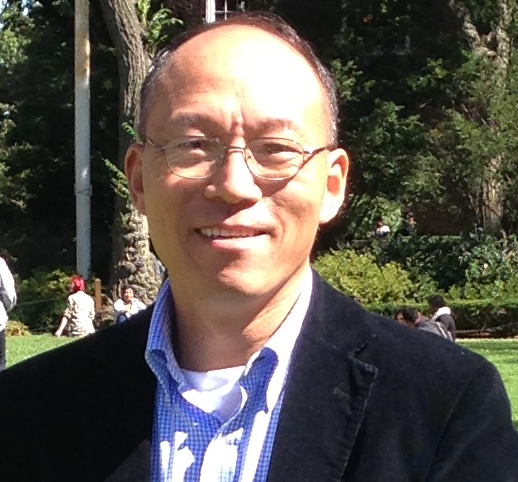
\includegraphics[scale=0.22]{res/zhou}
			\end{figure}
		
		\end{column}
	\end{columns}

\end{frame}